\documentclass[twoside]{book}

% Packages required by doxygen
\usepackage{fixltx2e}
\usepackage{calc}
\usepackage{doxygen}
\usepackage[export]{adjustbox} % also loads graphicx
\usepackage{graphicx}
\usepackage[utf8]{inputenc}
\usepackage{makeidx}
\usepackage{multicol}
\usepackage{multirow}
\PassOptionsToPackage{warn}{textcomp}
\usepackage{textcomp}
\usepackage[nointegrals]{wasysym}
\usepackage[table]{xcolor}

% Font selection
\usepackage[T1]{fontenc}
\usepackage[scaled=.90]{helvet}
\usepackage{courier}
\usepackage{amssymb}
\usepackage{sectsty}
\renewcommand{\familydefault}{\sfdefault}
\allsectionsfont{%
  \fontseries{bc}\selectfont%
  \color{darkgray}%
}
\renewcommand{\DoxyLabelFont}{%
  \fontseries{bc}\selectfont%
  \color{darkgray}%
}
\newcommand{\+}{\discretionary{\mbox{\scriptsize$\hookleftarrow$}}{}{}}

% Page & text layout
\usepackage{geometry}
\geometry{%
  a4paper,%
  top=2.5cm,%
  bottom=2.5cm,%
  left=2.5cm,%
  right=2.5cm%
}
\tolerance=750
\hfuzz=15pt
\hbadness=750
\setlength{\emergencystretch}{15pt}
\setlength{\parindent}{0cm}
\setlength{\parskip}{3ex plus 2ex minus 2ex}
\makeatletter
\renewcommand{\paragraph}{%
  \@startsection{paragraph}{4}{0ex}{-1.0ex}{1.0ex}{%
    \normalfont\normalsize\bfseries\SS@parafont%
  }%
}
\renewcommand{\subparagraph}{%
  \@startsection{subparagraph}{5}{0ex}{-1.0ex}{1.0ex}{%
    \normalfont\normalsize\bfseries\SS@subparafont%
  }%
}
\makeatother

% Headers & footers
\usepackage{fancyhdr}
\pagestyle{fancyplain}
\fancyhead[LE]{\fancyplain{}{\bfseries\thepage}}
\fancyhead[CE]{\fancyplain{}{}}
\fancyhead[RE]{\fancyplain{}{\bfseries\leftmark}}
\fancyhead[LO]{\fancyplain{}{\bfseries\rightmark}}
\fancyhead[CO]{\fancyplain{}{}}
\fancyhead[RO]{\fancyplain{}{\bfseries\thepage}}
\fancyfoot[LE]{\fancyplain{}{}}
\fancyfoot[CE]{\fancyplain{}{}}
\fancyfoot[RE]{\fancyplain{}{\bfseries\scriptsize Generated by Doxygen }}
\fancyfoot[LO]{\fancyplain{}{\bfseries\scriptsize Generated by Doxygen }}
\fancyfoot[CO]{\fancyplain{}{}}
\fancyfoot[RO]{\fancyplain{}{}}
\renewcommand{\footrulewidth}{0.4pt}
\renewcommand{\chaptermark}[1]{%
  \markboth{#1}{}%
}
\renewcommand{\sectionmark}[1]{%
  \markright{\thesection\ #1}%
}

% Indices & bibliography
\usepackage{natbib}
\usepackage[titles]{tocloft}
\setcounter{tocdepth}{3}
\setcounter{secnumdepth}{5}
\makeindex

% Hyperlinks (required, but should be loaded last)
\usepackage{ifpdf}
\ifpdf
  \usepackage[pdftex,pagebackref=true]{hyperref}
\else
  \usepackage[ps2pdf,pagebackref=true]{hyperref}
\fi
\hypersetup{%
  colorlinks=true,%
  linkcolor=blue,%
  citecolor=blue,%
  unicode%
}

% Custom commands
\newcommand{\clearemptydoublepage}{%
  \newpage{\pagestyle{empty}\cleardoublepage}%
}

\usepackage{caption}
\captionsetup{labelsep=space,justification=centering,font={bf},singlelinecheck=off,skip=4pt,position=top}

%===== C O N T E N T S =====

\begin{document}

% Titlepage & ToC
\hypersetup{pageanchor=false,
             bookmarksnumbered=true,
             pdfencoding=unicode
            }
\pagenumbering{alph}
\begin{titlepage}
\vspace*{7cm}
\begin{center}%
{\Large My Project }\\
\vspace*{1cm}
{\large Generated by Doxygen 1.8.12}\\
\end{center}
\end{titlepage}
\clearemptydoublepage
\pagenumbering{roman}
\tableofcontents
\clearemptydoublepage
\pagenumbering{arabic}
\hypersetup{pageanchor=true}

%--- Begin generated contents ---
\chapter{Hierarchical Index}
\section{Class Hierarchy}
This inheritance list is sorted roughly, but not completely, alphabetically\+:\begin{DoxyCompactList}
\item \contentsline{section}{Config}{\pageref{classConfig}}{}
\item Q\+Dialog\begin{DoxyCompactList}
\item \contentsline{section}{Dialog}{\pageref{classDialog}}{}
\end{DoxyCompactList}
\item \contentsline{section}{Universe\+Component}{\pageref{classUniverseComponent}}{}
\begin{DoxyCompactList}
\item \contentsline{section}{Universe\+Body}{\pageref{classUniverseBody}}{}
\item \contentsline{section}{Universe\+Composite}{\pageref{classUniverseComposite}}{}
\end{DoxyCompactList}
\item \contentsline{section}{Universe\+Component\+Factory}{\pageref{classUniverseComponentFactory}}{}
\item \contentsline{section}{Zodiac}{\pageref{classZodiac}}{}
\end{DoxyCompactList}

\chapter{Class Index}
\section{Class List}
Here are the classes, structs, unions and interfaces with brief descriptions\+:\begin{DoxyCompactList}
\item\contentsline{section}{\hyperlink{classConfig}{Config} }{\pageref{classConfig}}{}
\item\contentsline{section}{\hyperlink{classDialog}{Dialog} }{\pageref{classDialog}}{}
\item\contentsline{section}{\hyperlink{classUniverseBody}{Universe\+Body} }{\pageref{classUniverseBody}}{}
\item\contentsline{section}{\hyperlink{classUniverseComponent}{Universe\+Component} }{\pageref{classUniverseComponent}}{}
\item\contentsline{section}{\hyperlink{classUniverseComponentFactory}{Universe\+Component\+Factory} }{\pageref{classUniverseComponentFactory}}{}
\item\contentsline{section}{\hyperlink{classUniverseComposite}{Universe\+Composite} }{\pageref{classUniverseComposite}}{}
\item\contentsline{section}{\hyperlink{classZodiac}{Zodiac} }{\pageref{classZodiac}}{}
\end{DoxyCompactList}

\chapter{Class Documentation}
\hypertarget{classConfig}{}\section{Config Class Reference}
\label{classConfig}\index{Config@{Config}}
\subsection*{Public Member Functions}
\begin{DoxyCompactItemize}
\item 
void {\bfseries read} (const std\+::string \&path)\hypertarget{classConfig_a73524943ef4dadd5e0dfd7ce118c26bf}{}\label{classConfig_a73524943ef4dadd5e0dfd7ce118c26bf}

\item 
\hyperlink{classUniverseComponent}{Universe\+Component} $\ast$ {\bfseries parse\+Universe\+Blocks} ()\hypertarget{classConfig_a0d9929daff1f0313c37112924532cc2e}{}\label{classConfig_a0d9929daff1f0313c37112924532cc2e}

\item 
std\+::list$<$ \hyperlink{classZodiac}{Zodiac} $>$ $\ast$ {\bfseries parse\+Zodiac\+Blocks} ()\hypertarget{classConfig_a7f6dd6aff9f561fb14f884eca32b1c14}{}\label{classConfig_a7f6dd6aff9f561fb14f884eca32b1c14}

\item 
double {\bfseries get\+Frames\+Per\+Second} () const\hypertarget{classConfig_a46fd73144acb372b17e3f8e81198c8a8}{}\label{classConfig_a46fd73144acb372b17e3f8e81198c8a8}

\item 
int {\bfseries get\+Physics\+Step\+Size} () const\hypertarget{classConfig_a7a55c8628d74484b182d0d9895e2568a}{}\label{classConfig_a7a55c8628d74484b182d0d9895e2568a}

\item 
int {\bfseries get\+Overcalculate\+Physics\+Amount} () const\hypertarget{classConfig_a0b00e58caf959e6ef2c19c96d5798b37}{}\label{classConfig_a0b00e58caf959e6ef2c19c96d5798b37}

\item 
double {\bfseries get\+Distance\+Scale} () const\hypertarget{classConfig_a63a31c1c57918c01ee3fb8134c427df1}{}\label{classConfig_a63a31c1c57918c01ee3fb8134c427df1}

\item 
double {\bfseries get\+Radius\+Scale} () const\hypertarget{classConfig_a6fe4db97750a726f288d6d4511857dbc}{}\label{classConfig_a6fe4db97750a726f288d6d4511857dbc}

\item 
bool {\bfseries get\+Use\+Log\+Radius} () const\hypertarget{classConfig_a62181b58313707d1c660ad451e92ba0d}{}\label{classConfig_a62181b58313707d1c660ad451e92ba0d}

\item 
double {\bfseries get\+Log\+Point\+Radius} () const\hypertarget{classConfig_a7b666265a00af475c965650fd6b71302}{}\label{classConfig_a7b666265a00af475c965650fd6b71302}

\end{DoxyCompactItemize}
\subsection*{Static Public Member Functions}
\begin{DoxyCompactItemize}
\item 
static \hyperlink{classConfig}{Config} $\ast$ {\bfseries get\+Instance} ()\hypertarget{classConfig_af7d6f89fc34627f15523df0b62acd7e5}{}\label{classConfig_af7d6f89fc34627f15523df0b62acd7e5}

\end{DoxyCompactItemize}


The documentation for this class was generated from the following files\+:\begin{DoxyCompactItemize}
\item 
config.\+h\item 
config.\+cpp\end{DoxyCompactItemize}

\hypertarget{classDialog}{}\section{Dialog Class Reference}
\label{classDialog}\index{Dialog@{Dialog}}
Inheritance diagram for Dialog\+:\begin{figure}[H]
\begin{center}
\leavevmode
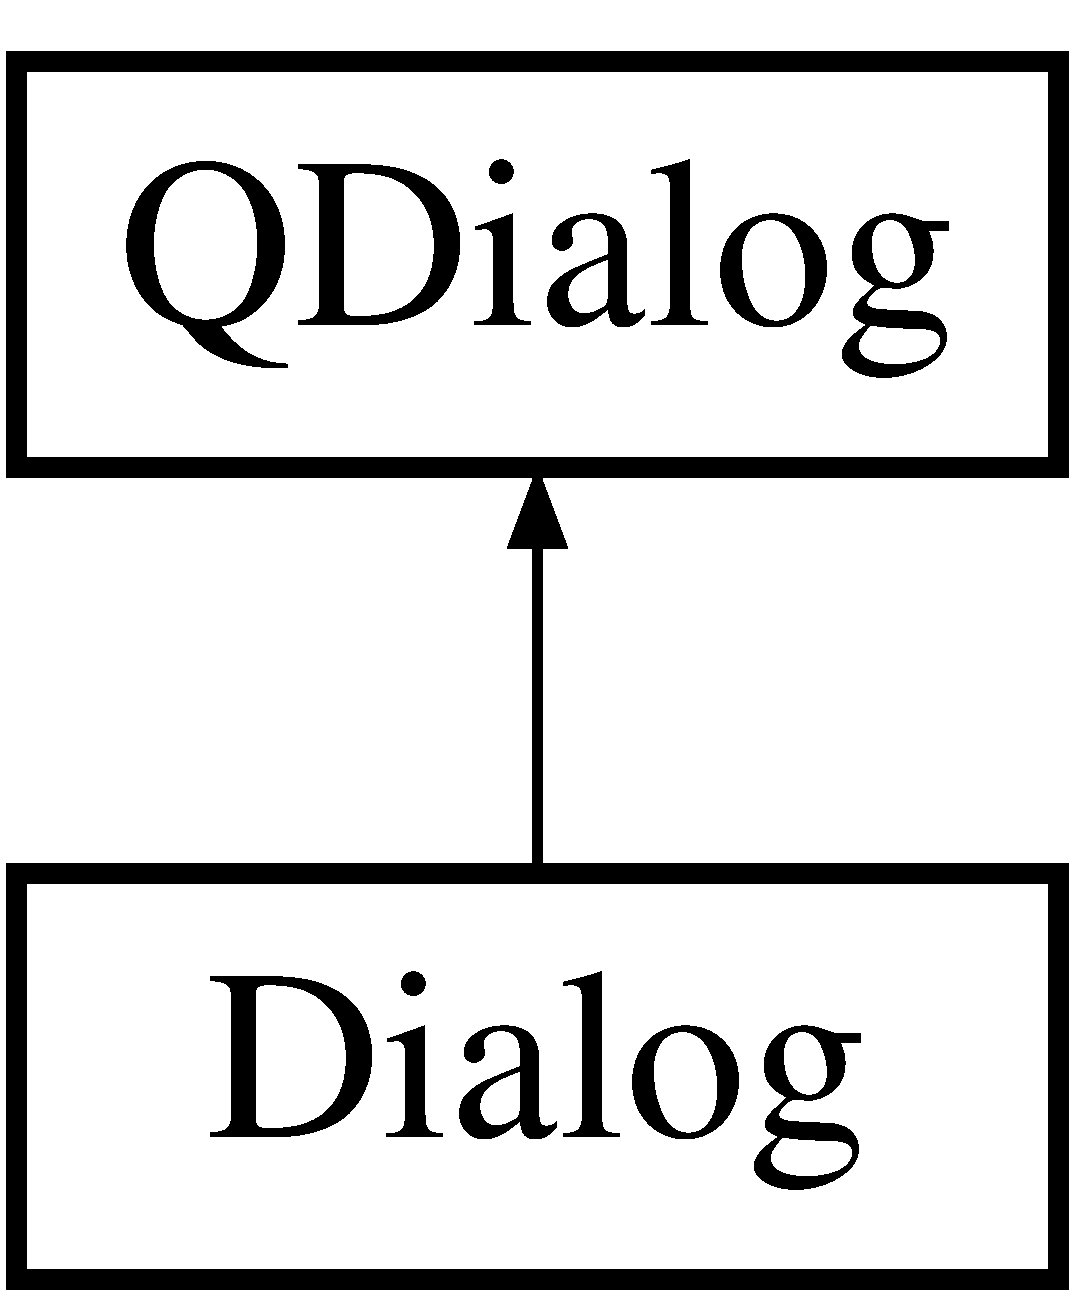
\includegraphics[height=2.000000cm]{classDialog}
\end{center}
\end{figure}
\subsection*{Public Member Functions}
\begin{DoxyCompactItemize}
\item 
{\bfseries Dialog} (Q\+Widget $\ast$parent=0)\hypertarget{classDialog_acfa2063f9f962d394c6a645b6e7e08d8}{}\label{classDialog_acfa2063f9f962d394c6a645b6e7e08d8}

\end{DoxyCompactItemize}


The documentation for this class was generated from the following files\+:\begin{DoxyCompactItemize}
\item 
dialog.\+h\item 
dialog.\+cpp\end{DoxyCompactItemize}

\hypertarget{classUniverseBody}{}\section{Universe\+Body Class Reference}
\label{classUniverseBody}\index{Universe\+Body@{Universe\+Body}}
Inheritance diagram for Universe\+Body\+:\begin{figure}[H]
\begin{center}
\leavevmode
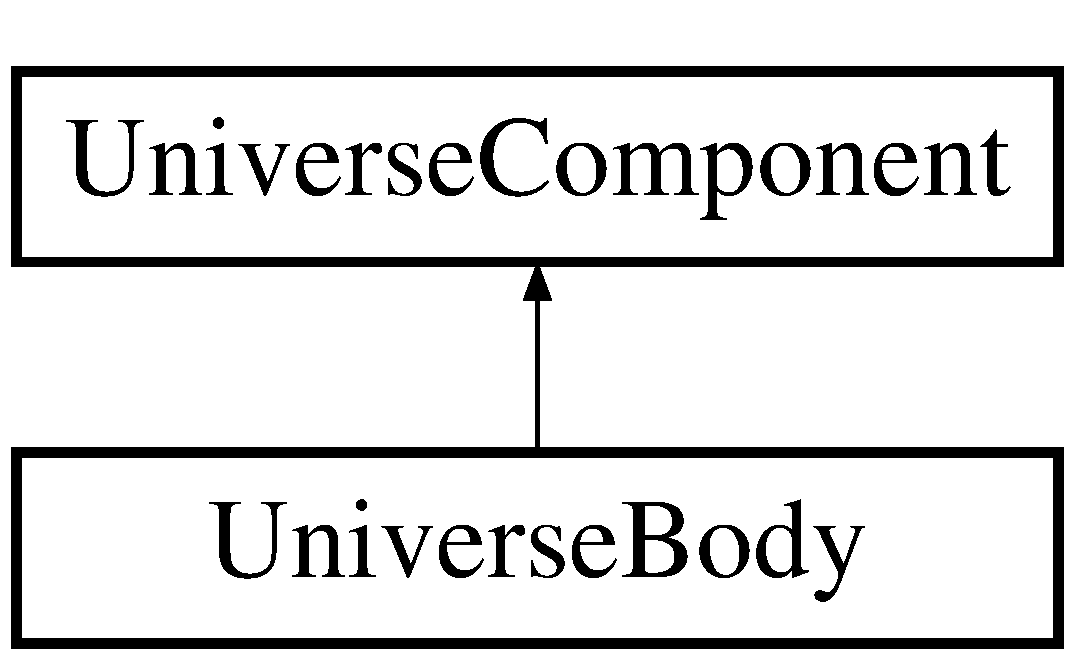
\includegraphics[height=2.000000cm]{classUniverseBody}
\end{center}
\end{figure}
\subsection*{Public Member Functions}
\begin{DoxyCompactItemize}
\item 
{\bfseries Universe\+Body} (Universe\+Component\+Type type, const std\+::string \&name, const std\+::string \&parent\+Name=\char`\"{}\char`\"{})\hypertarget{classUniverseBody_a495e1daf0ebb87f016a4240a9c1e1808}{}\label{classUniverseBody_a495e1daf0ebb87f016a4240a9c1e1808}

\item 
virtual void {\bfseries render} (Q\+Painter \&painter) const\hypertarget{classUniverseBody_a70e698b61bea240d49eb8e7ab8b3adcc}{}\label{classUniverseBody_a70e698b61bea240d49eb8e7ab8b3adcc}

\item 
virtual void {\bfseries render\+Label} (Q\+Painter \&painter) const\hypertarget{classUniverseBody_ac715dabc3f3ad74885eab48641f48349}{}\label{classUniverseBody_ac715dabc3f3ad74885eab48641f48349}

\item 
virtual void {\bfseries add\+Attraction\+To} (\hyperlink{classUniverseBody}{Universe\+Body} \&body) const\hypertarget{classUniverseBody_a75be4fe3635ad3fabd32a91e1529d91a}{}\label{classUniverseBody_a75be4fe3635ad3fabd32a91e1529d91a}

\item 
virtual void {\bfseries add\+Attraction\+From} (const \hyperlink{classUniverseComponent}{Universe\+Component} \&component)\hypertarget{classUniverseBody_a1e02b10cac430619e38ed85693e5445b}{}\label{classUniverseBody_a1e02b10cac430619e38ed85693e5445b}

\item 
virtual void {\bfseries reset\+Forces} ()\hypertarget{classUniverseBody_a284d6976b43911bfdb58e86beabb5c46}{}\label{classUniverseBody_a284d6976b43911bfdb58e86beabb5c46}

\item 
virtual void {\bfseries update\+Position} (int timestep)\hypertarget{classUniverseBody_a5a0ed5719f40137bc0ed135fee91de8e}{}\label{classUniverseBody_a5a0ed5719f40137bc0ed135fee91de8e}

\item 
void {\bfseries convert\+Relative\+To\+Absolute} (double xp, double yp, double xv, double yv)\hypertarget{classUniverseBody_a3d63022b51f35c24d016700921c50841}{}\label{classUniverseBody_a3d63022b51f35c24d016700921c50841}

\item 
const Q\+Color \& {\bfseries get\+Color} () const\hypertarget{classUniverseBody_a317a6bb602fa64d6bc672bafb493ecb6}{}\label{classUniverseBody_a317a6bb602fa64d6bc672bafb493ecb6}

\item 
double {\bfseries get\+PositionX} () const\hypertarget{classUniverseBody_a4bad5fe82362af021b3798f0739df4ef}{}\label{classUniverseBody_a4bad5fe82362af021b3798f0739df4ef}

\item 
double {\bfseries get\+PositionY} () const\hypertarget{classUniverseBody_a6ae3f80f3cad5a943ff40622cf81fbdc}{}\label{classUniverseBody_a6ae3f80f3cad5a943ff40622cf81fbdc}

\item 
double {\bfseries get\+Mass} () const\hypertarget{classUniverseBody_a45d334390363d63200ff668f524477b0}{}\label{classUniverseBody_a45d334390363d63200ff668f524477b0}

\item 
void {\bfseries add\+Force} (double x, double y)\hypertarget{classUniverseBody_aae9f301e3dffe3c4d5ce4ce1c2bc6591}{}\label{classUniverseBody_aae9f301e3dffe3c4d5ce4ce1c2bc6591}

\item 
void {\bfseries set\+Position} (const double x, const double y)\hypertarget{classUniverseBody_aa15ba5311d80474c6f74e2fbbf39bd54}{}\label{classUniverseBody_aa15ba5311d80474c6f74e2fbbf39bd54}

\item 
void {\bfseries set\+Velocity} (const double x, const double y)\hypertarget{classUniverseBody_ae34bed5731be5dfba2a86f1ee5fa40ca}{}\label{classUniverseBody_ae34bed5731be5dfba2a86f1ee5fa40ca}

\item 
void {\bfseries set\+Radius} (const double \&radius)\hypertarget{classUniverseBody_a9c609437abfacd5bfb3772e6d32fb0fb}{}\label{classUniverseBody_a9c609437abfacd5bfb3772e6d32fb0fb}

\item 
void {\bfseries set\+Mass} (const double \&mass)\hypertarget{classUniverseBody_ad01381589096b71035595502829ed039}{}\label{classUniverseBody_ad01381589096b71035595502829ed039}

\item 
void {\bfseries set\+Color} (const Q\+Color \&color)\hypertarget{classUniverseBody_a464502083e736aa7472d8ea3c64c695e}{}\label{classUniverseBody_a464502083e736aa7472d8ea3c64c695e}

\end{DoxyCompactItemize}


The documentation for this class was generated from the following files\+:\begin{DoxyCompactItemize}
\item 
universebody.\+h\item 
universebody.\+cpp\end{DoxyCompactItemize}

\hypertarget{classUniverseComponent}{}\section{Universe\+Component Class Reference}
\label{classUniverseComponent}\index{Universe\+Component@{Universe\+Component}}
Inheritance diagram for Universe\+Component\+:\begin{figure}[H]
\begin{center}
\leavevmode
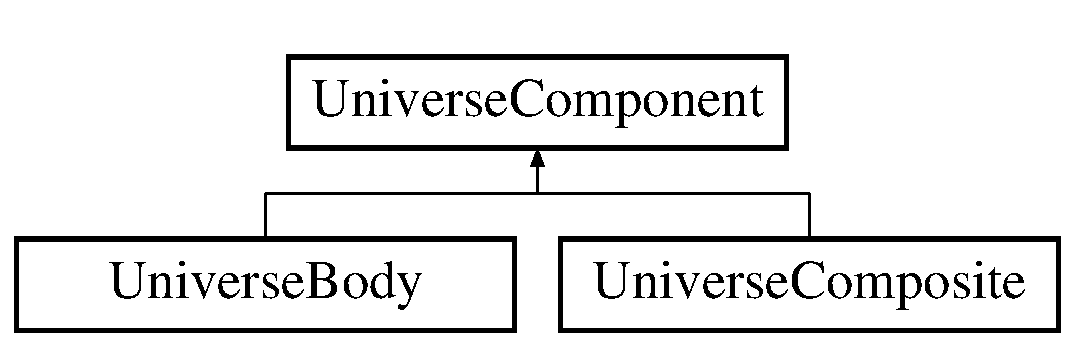
\includegraphics[height=2.000000cm]{classUniverseComponent}
\end{center}
\end{figure}
\subsection*{Public Member Functions}
\begin{DoxyCompactItemize}
\item 
{\bfseries Universe\+Component} (Universe\+Component\+Type type, const std\+::string \&name, const std\+::string \&parent\+Name=\char`\"{}\char`\"{})\hypertarget{classUniverseComponent_ae27a92b369e5eab3016d1a570766a974}{}\label{classUniverseComponent_ae27a92b369e5eab3016d1a570766a974}

\item 
virtual void {\bfseries render} (Q\+Painter \&painter) const =0\hypertarget{classUniverseComponent_ab5a74e2a809f24509770c85fcfb4f2c5}{}\label{classUniverseComponent_ab5a74e2a809f24509770c85fcfb4f2c5}

\item 
virtual void {\bfseries render\+Label} (Q\+Painter \&painter) const =0\hypertarget{classUniverseComponent_aa35a0218177fa8b0852cf041dbabd43a}{}\label{classUniverseComponent_aa35a0218177fa8b0852cf041dbabd43a}

\item 
virtual void {\bfseries add\+Attraction\+To} (\hyperlink{classUniverseBody}{Universe\+Body} \&other) const =0\hypertarget{classUniverseComponent_a1bee459df6e2e4ba2bdfee7ce0db1b1f}{}\label{classUniverseComponent_a1bee459df6e2e4ba2bdfee7ce0db1b1f}

\item 
virtual void {\bfseries reset\+Forces} ()=0\hypertarget{classUniverseComponent_a487cb9ffee239439d73216e413890c66}{}\label{classUniverseComponent_a487cb9ffee239439d73216e413890c66}

\item 
virtual void {\bfseries add\+Attraction\+From} (const \hyperlink{classUniverseComponent}{Universe\+Component} \&component)=0\hypertarget{classUniverseComponent_ad7d582f1e3cc26b30b25920820f006d4}{}\label{classUniverseComponent_ad7d582f1e3cc26b30b25920820f006d4}

\item 
virtual void {\bfseries update\+Position} (int timestep)=0\hypertarget{classUniverseComponent_aac0500ee56b3aecbdcddc663efc96aed}{}\label{classUniverseComponent_aac0500ee56b3aecbdcddc663efc96aed}

\item 
virtual void {\bfseries convert\+Relative\+To\+Absolute} (double xp, double yp, double xv, double yv)=0\hypertarget{classUniverseComponent_adee9b6dda24030f697c1c9dc76a066f9}{}\label{classUniverseComponent_adee9b6dda24030f697c1c9dc76a066f9}

\item 
void {\bfseries set\+Name} (const std\+::string \&name)\hypertarget{classUniverseComponent_ac69d32c49d432e23a1435828a3e97d4e}{}\label{classUniverseComponent_ac69d32c49d432e23a1435828a3e97d4e}

\item 
const std\+::string \& {\bfseries get\+Name} () const\hypertarget{classUniverseComponent_a7115f8b2b4f1877d39e4280d889d5bc5}{}\label{classUniverseComponent_a7115f8b2b4f1877d39e4280d889d5bc5}

\item 
const std\+::string \& {\bfseries get\+Parent\+Name} () const\hypertarget{classUniverseComponent_a62a75461599a15b5c28e0daca8669b29}{}\label{classUniverseComponent_a62a75461599a15b5c28e0daca8669b29}

\item 
Universe\+Component\+Type {\bfseries get\+Type} () const\hypertarget{classUniverseComponent_ad601325204de75c91829655f3b735f74}{}\label{classUniverseComponent_ad601325204de75c91829655f3b735f74}

\end{DoxyCompactItemize}


The documentation for this class was generated from the following file\+:\begin{DoxyCompactItemize}
\item 
universecomponent.\+h\end{DoxyCompactItemize}

\hypertarget{classUniverseComponentFactory}{}\section{Universe\+Component\+Factory Class Reference}
\label{classUniverseComponentFactory}\index{Universe\+Component\+Factory@{Universe\+Component\+Factory}}
\subsection*{Public Member Functions}
\begin{DoxyCompactItemize}
\item 
virtual \hyperlink{classUniverseComponent}{Universe\+Component} $\ast$ {\bfseries create\+Universe\+Component} (const std\+::unordered\+\_\+map$<$ std\+::string, std\+::string $>$ \&block) const\hypertarget{classUniverseComponentFactory_a79ce139450c104c1c01aeca0ddba27b0}{}\label{classUniverseComponentFactory_a79ce139450c104c1c01aeca0ddba27b0}

\end{DoxyCompactItemize}


The documentation for this class was generated from the following files\+:\begin{DoxyCompactItemize}
\item 
universecomponentfactory.\+h\item 
universecomponentfactory.\+cpp\end{DoxyCompactItemize}

\hypertarget{classUniverseComposite}{}\section{Universe\+Composite Class Reference}
\label{classUniverseComposite}\index{Universe\+Composite@{Universe\+Composite}}
Inheritance diagram for Universe\+Composite\+:\begin{figure}[H]
\begin{center}
\leavevmode
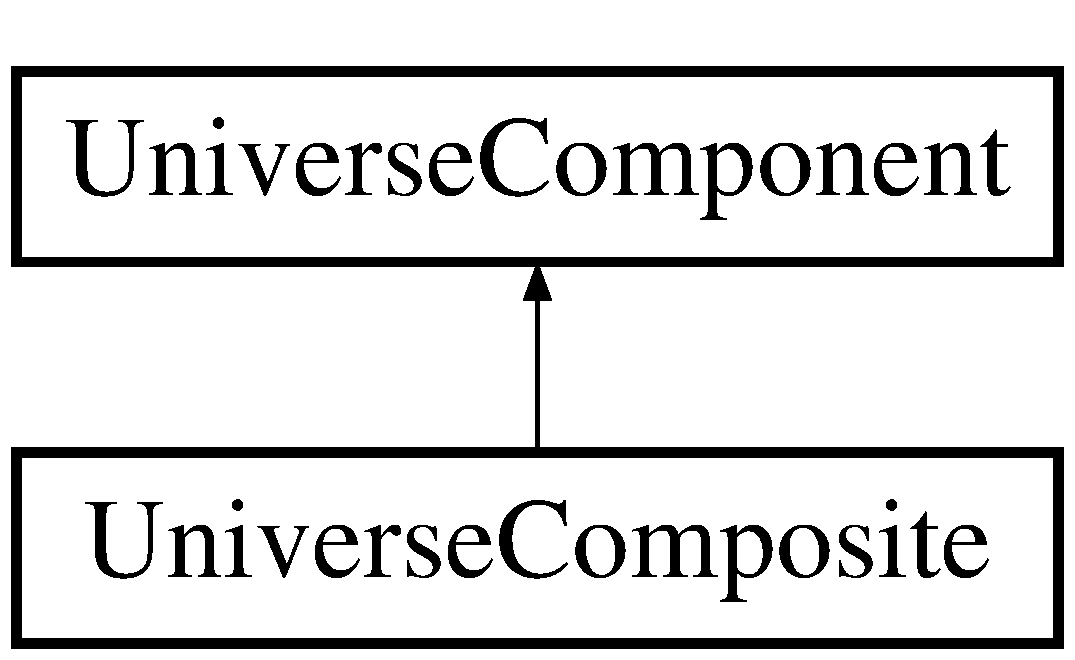
\includegraphics[height=2.000000cm]{classUniverseComposite}
\end{center}
\end{figure}
\subsection*{Public Member Functions}
\begin{DoxyCompactItemize}
\item 
{\bfseries Universe\+Composite} (Universe\+Component\+Type type, const std\+::string \&name, const std\+::string \&parent\+Name=\char`\"{}\char`\"{})\hypertarget{classUniverseComposite_a1d502725a50d0bb57fc82dd26af04404}{}\label{classUniverseComposite_a1d502725a50d0bb57fc82dd26af04404}

\item 
virtual void {\bfseries add} (\hyperlink{classUniverseComponent}{Universe\+Component} $\ast$component)\hypertarget{classUniverseComposite_a688fc563c75b5409694b87b3e93f536f}{}\label{classUniverseComposite_a688fc563c75b5409694b87b3e93f536f}

\item 
virtual void {\bfseries render} (Q\+Painter \&painter) const\hypertarget{classUniverseComposite_a6d4cc7a4d02f3a0caedc13da32478add}{}\label{classUniverseComposite_a6d4cc7a4d02f3a0caedc13da32478add}

\item 
virtual void {\bfseries render\+Label} (Q\+Painter \&painter) const\hypertarget{classUniverseComposite_a288713a094824e0bea8f66fa81e9735b}{}\label{classUniverseComposite_a288713a094824e0bea8f66fa81e9735b}

\item 
virtual void {\bfseries add\+Attraction\+To} (\hyperlink{classUniverseBody}{Universe\+Body} \&other) const\hypertarget{classUniverseComposite_af31da7bdf116c0842b8688d03798e032}{}\label{classUniverseComposite_af31da7bdf116c0842b8688d03798e032}

\item 
virtual void {\bfseries reset\+Forces} ()\hypertarget{classUniverseComposite_a2129af893c2246c195885d33ad35b3f8}{}\label{classUniverseComposite_a2129af893c2246c195885d33ad35b3f8}

\item 
virtual void {\bfseries add\+Attraction\+From} (const \hyperlink{classUniverseComponent}{Universe\+Component} \&component)\hypertarget{classUniverseComposite_a693ebf330331eb02aee9a899a6ed9931}{}\label{classUniverseComposite_a693ebf330331eb02aee9a899a6ed9931}

\item 
virtual void {\bfseries update\+Position} (int timestep)\hypertarget{classUniverseComposite_a06dcff451e2dfc3886555593a2e462d2}{}\label{classUniverseComposite_a06dcff451e2dfc3886555593a2e462d2}

\item 
void {\bfseries set\+Position} (double x, double y)\hypertarget{classUniverseComposite_ade4bd314e57e8b30bd33f7c3f164edef}{}\label{classUniverseComposite_ade4bd314e57e8b30bd33f7c3f164edef}

\item 
void {\bfseries set\+Velocity} (double x, double y)\hypertarget{classUniverseComposite_a1dcbef25b73e189934e6cccb0bc2ef2e}{}\label{classUniverseComposite_a1dcbef25b73e189934e6cccb0bc2ef2e}

\item 
void {\bfseries convert\+Relative\+To\+Absolute} (double xp, double yp, double xv, double yv)\hypertarget{classUniverseComposite_a0410ce4d77d4b408148a9f51647d223f}{}\label{classUniverseComposite_a0410ce4d77d4b408148a9f51647d223f}

\end{DoxyCompactItemize}


The documentation for this class was generated from the following files\+:\begin{DoxyCompactItemize}
\item 
universecomposite.\+h\item 
universecomposite.\+cpp\end{DoxyCompactItemize}

\hypertarget{classZodiac}{}\section{Zodiac Class Reference}
\label{classZodiac}\index{Zodiac@{Zodiac}}
\subsection*{Public Member Functions}
\begin{DoxyCompactItemize}
\item 
virtual void {\bfseries render} (Q\+Painter \&painter) const\hypertarget{classZodiac_afd9c80e90ed00d1302ab70d97aabc40c}{}\label{classZodiac_afd9c80e90ed00d1302ab70d97aabc40c}

\item 
virtual void {\bfseries add} (\hyperlink{classUniverseBody}{Universe\+Body} $\ast$from, \hyperlink{classUniverseBody}{Universe\+Body} $\ast$to)\hypertarget{classZodiac_a2bb308851769d1657b2c02e9f2b4e553}{}\label{classZodiac_a2bb308851769d1657b2c02e9f2b4e553}

\end{DoxyCompactItemize}


The documentation for this class was generated from the following files\+:\begin{DoxyCompactItemize}
\item 
zodiac.\+h\item 
zodiac.\+cpp\end{DoxyCompactItemize}

%--- End generated contents ---

% Index
\backmatter
\newpage
\phantomsection
\clearemptydoublepage
\addcontentsline{toc}{chapter}{Index}
\printindex

\end{document}
